\documentclass[12pt,a4paper]{article}
\usepackage{rmpackages}
\usepackage{rmtemplaterapport}

\bibliographystyle{custom-bib/thesis}
\usepackage{bibentry}
\usepackage{pdfpages}


\title{L'expérience de Benjamin Franklin... Et Rayleigh, Pockels, Devaux, et Langmuir}
\author{Rémi Metzdorff}
\date{\today}

\begin{document}

\maketitle

\tableofcontents
\newpage

\section*{Introduction}
\addcontentsline{toc}{section}{Introduction}

\section{Les origines}

\cite{Franklin1773a}, Correspondance entre Franklin et Brownrigg.
L'expérience légendaire mais lui s'en cogne de la l'épaisseur de la couche d'huile.
Il remarque simplement que ça calme les vagues et que l'huile s'étend beaucoup.

\cite{Rayleigh1890a}, Measurements of the amount of oil necessary in order to check the motions of camphor upon water.
Il mesure la masse d'huile nécessaire pour arrêter le mouvement de camphre sur un grand bac d'eau et en déduit l'épaisseur du film correspondant.

\cite{Pockels1891}, Surface Tension.
Diverses expériences sur la tension de surface dans une lettre envoyée à Rayleigh.
Surface normale : la tension de surface ne dépend pas de l'aire de la surface d'eau dans son dispositif.
Surface anormale : a tension de surface dépend fortement de l'aire.
Courant de solution.
Solubilité de surface très élevée.

\cite{Rayleigh1892} : Experiments upon surface-films.
On comprend pourquoi ils utilisent le camphre comme indicateur de la tension de surface.
Il est dit que lorsque le camphre ne bouge plus, la tension de surface est en dessous de 0{,}72 fois celle de l'eau. 

\cite{Pockels1894} : On the Spreading of Oil upon Water.
Elle décrit très bien ce qu'il se passe si on ajoute de l'huile sur une surface saturée, même si cela semble déjà bien connu (\cite{Rayleigh1892}).

\cite{Rayleigh1899} : Investigations in capillarity.
Reproduction des expériences de Pockels (\cite{Pockels1891}), mesure de la tension de surface d'une eau contaminé avec de l'huile avec un tensiomètre à plaque de Wilhelmy.
Discussion sur l'état normal et l'état anormal de la surface.
Évoque la nécessité d'utiliser la notion de molécule pour expliquer la transition.
Discrétisation des valeurs de tension superficielle suivant le nombre de couches monomoléculaires.
Il suppose une couche monomoléculaire et en déduit le diamètre d'une molécule d'huile : \unit{1}{nm}.

\cite{Devaux1904} : Comparaison de l'épaisseur critique des lames très minces avec le diamètre théorique des molécules.
Tout est dans le titre, il semblerai qu'il soit le premier à comparer la hauteur du film avec la taille théorique des molécules.
Celle-ci est fournie grâce aux travaux de Nernst qui se base sur des considérations thermodynamiques (théorie cinétique des gaz : libre parcours moyen des molécules, section efficace) pour calculer les grandeurs moléculaires.

1913 : Marcelin, Epaisseur des couches très minces à la surface de l'eau, Diplôme d'études sup., Paris (1913), Ann. de Phys. (1913). Texte non trouvé

\cite{Langmuir1917} : The constitution and fundamental properties of solids and liquids. II. Liquids.
En plus d'une revue très claire des apports de Rayleigh, Pockels, Devaux et Marcelin, il évoque les raisons qui poussent le film d'huile à s'étendre et discute l'orientation des molécules d'huile à la surface de l'eau.
Ses considération théoriques sur les propriétés hydrophiles du groupement carboxyle (et de la double liaison) et hydrophobe des chaines carbonées sont suivies d'expériences permettant de déterminer à la fois la longueur des molécules d'huiles (l'épaisseur du film d'huile) et leur diamètre (en estimant la surface occupée par chaque molécule connaissant le nombre de molécule déposé).
Il tord aussi le coup aux hypothèses de film bi-moléculaire proposés par Rayleigh et Marcelin en invoquant la notamment souplesse des chaines carbonées.

\cite{BiolinScientific2011} : Fabricating Highly Organized Nanoparticle Thin Films.
Aujourd'hui, le procédé de déposition Langmuir-Blodgett permet d'obtenir des film mono ou multicouche de composés variés.

\section{Analyse de l'expérience en seconde}

\subsection{Dans le programme}

\subsection{L'activité}

\subsection{Analyse a priori}

\subsection{Analyse a posteriori}

\section{Réalisation expérimentale}

Difficile d'avoir une couche mono-moléculaire.
Il faut :
\begin{itemize}
\item soit un grand étang ;
\item soit une très petite quantité d'huile : il faut la dissoudre dans un solvant volatil.
\end{itemize}
Historiquement, c'est le benzène (appelé benzine à l'époque) mais ça va pas trop toxique.
Dans les protocoles plus modernes, on utilise de l'essence de térébenthine mais ça va pas c'est trop peu volatil et toxique.
Il faudrait essayer l'acétate d'éthyle : aussi volatil que le benzène mais beaucoup moins toxique.
 

\begin{table}
\center
\begin{tabular}{l|c|l}
\textbf{Composé} & $P_\mathrm{sat}^{\unit{20}{\celsius}}$ (mbar) & \textbf{Toxicité} \\
\hline \hline
Éther diéthylique & 586 & H224, H302, H336 \\
Cyclohexane & 127 & H225, H304, H315, H336, H410 \\
Benzène & 100 & H225, H304, H315, H319, H340, H350, H372 \\
Acétate d'éthyle & 100 & H225, H319, H336 \\
Éthanol & 58 & H225 \\
Essence de térébenthine  & 5{,}35 &  H226, H302, H304, H312, H315, H317, H319, ... \\
\end{tabular}
\caption{Éther diéthylique : trop inflammable. Cyclohexane : trop toxique. Benzène : trop toxique. Acétate d'éthyle : il faut vérifier que ça fonctionne. Éthanol : soluble dans l'eau, a priori huile non soluble dedans, seulement l'acide oléique. Essence de térébenthine : peu volatil et toxique.}
\end{table}

\section*{Conclusion}
\addcontentsline{toc}{section}{Conclusion}

\newpage
\appendix

\bibliography{biblio.bib}
\addcontentsline{toc}{section}{Références}

\newpage
\section{Document élève}
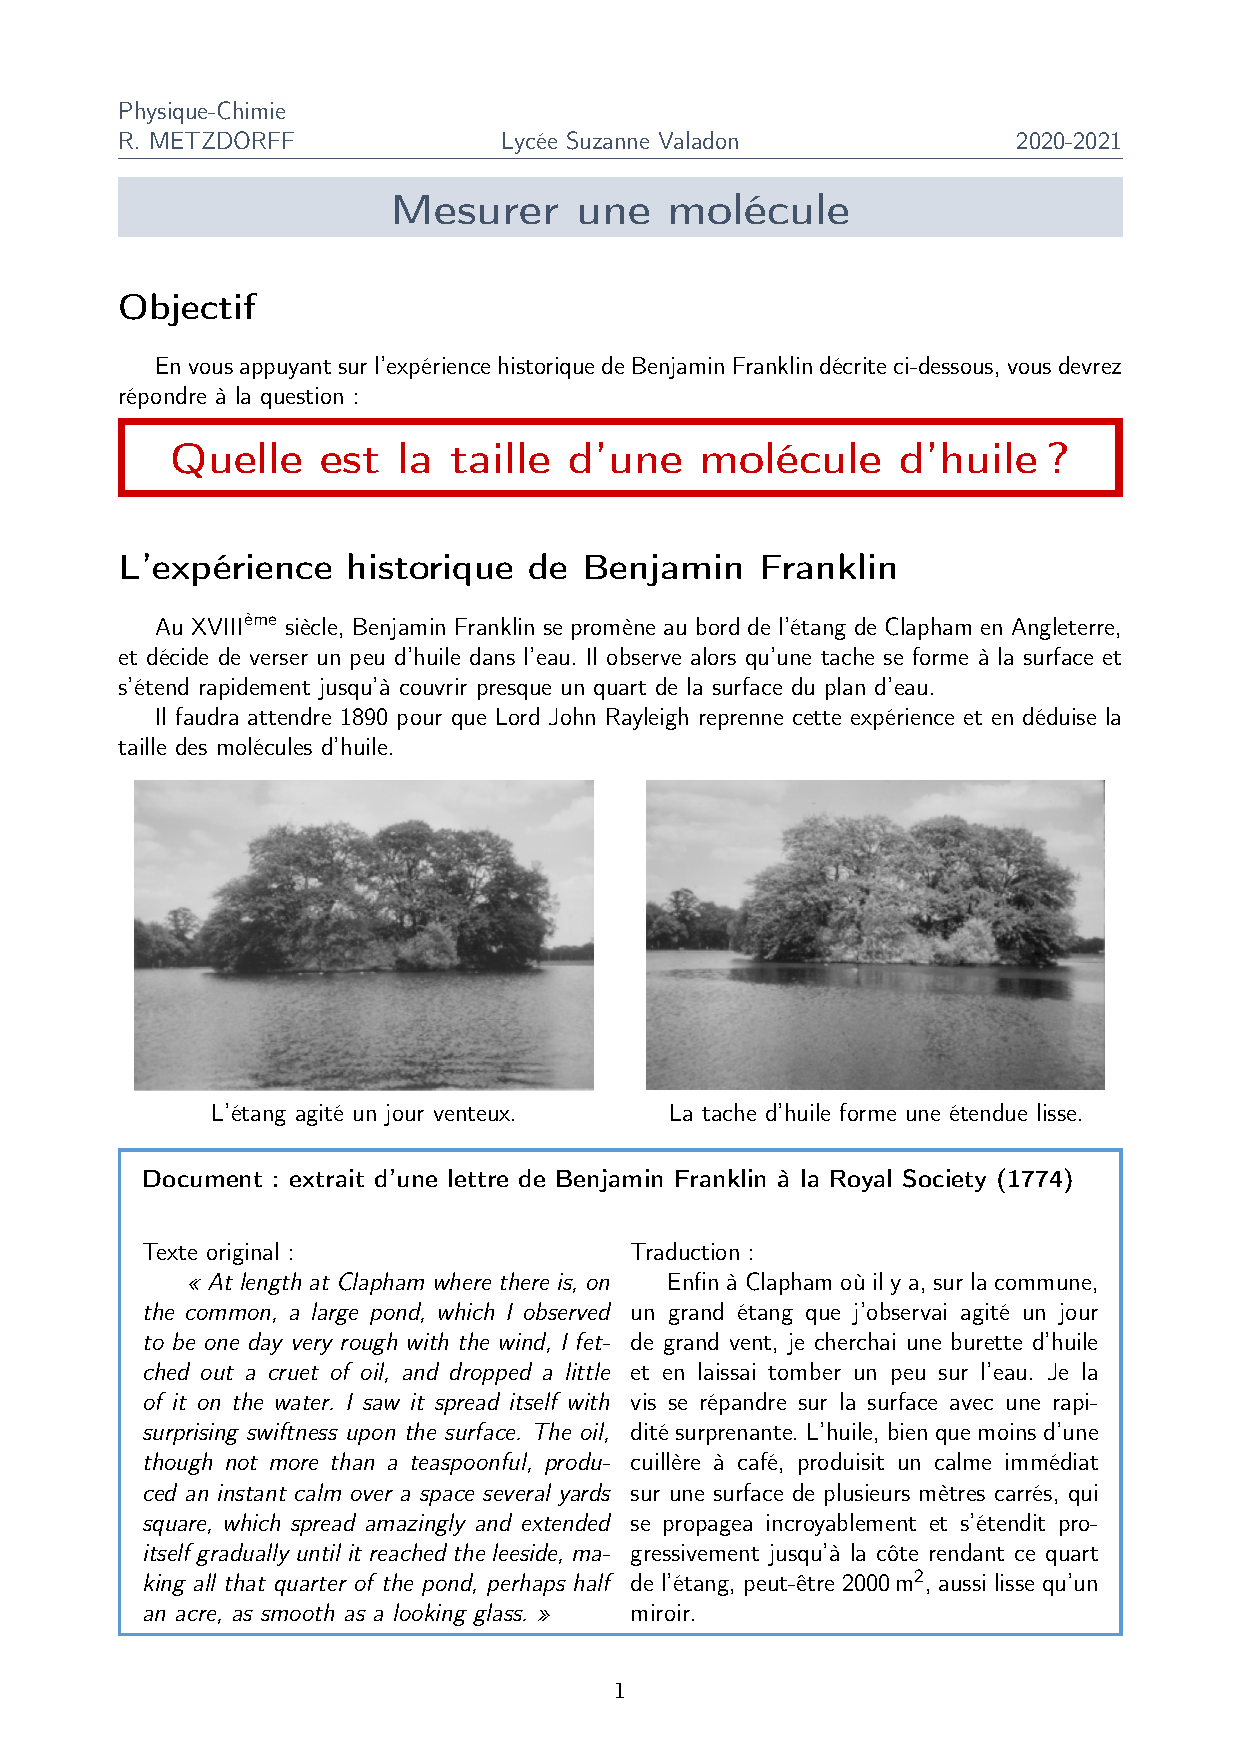
\includepdf[pages=-]{tp_franklin_v1.pdf}

\newpage
\section{Suite}


\end{document}